\chapter{Metodología}
\label{cap:metodologia}

Este capítulo cuenta cómo medimos réplicas rígidas de peces a partir de fotografías tomadas a través de una pecera. La investigación es aplicada, cuantitativa y usa un diseño experimental pareado. Pareado significa que cada imagen, con sus mismos puntos anatómicos, pasó por los cuatro métodos de conversión métrica: cualquier diferencia entre ellos se debe al método y no a la foto.

\section{Tipo de investigación, enfoque, población y muestra}
\label{sec:diseno}

Se trata de una investigación aplicada, cuantitativa y experimental, con diseño pareado: cada unidad experimental recibe los cuatro tratamientos (A, \Aprime, B y C) sobre la misma observación. La población objetivo son las imágenes de peces tomadas a través de un vidrio plano con una cámara externa. La muestra no es probabilística: son las 72 imágenes de las seis réplicas rígidas disponibles, fotografiadas a cuatro profundidades con tres capturas por condición.

La unidad experimental es una réplica rígida de pez, y la unidad de observación, una medición obtenida de una fotografía. Usamos seis réplicas, R1--R6, impresas en PLA y de tamaños distintos (Figura~\ref{fig:3-1}). La especie que imitan no es una variable del estudio: buscamos variedad de formas y longitudes. Medimos con calibre las dimensiones de referencia de cada réplica y las registramos en el archivo maestro del experimento (Tabla~\ref{tab:replicas}).

\begin{figure}[htbp]
\centering
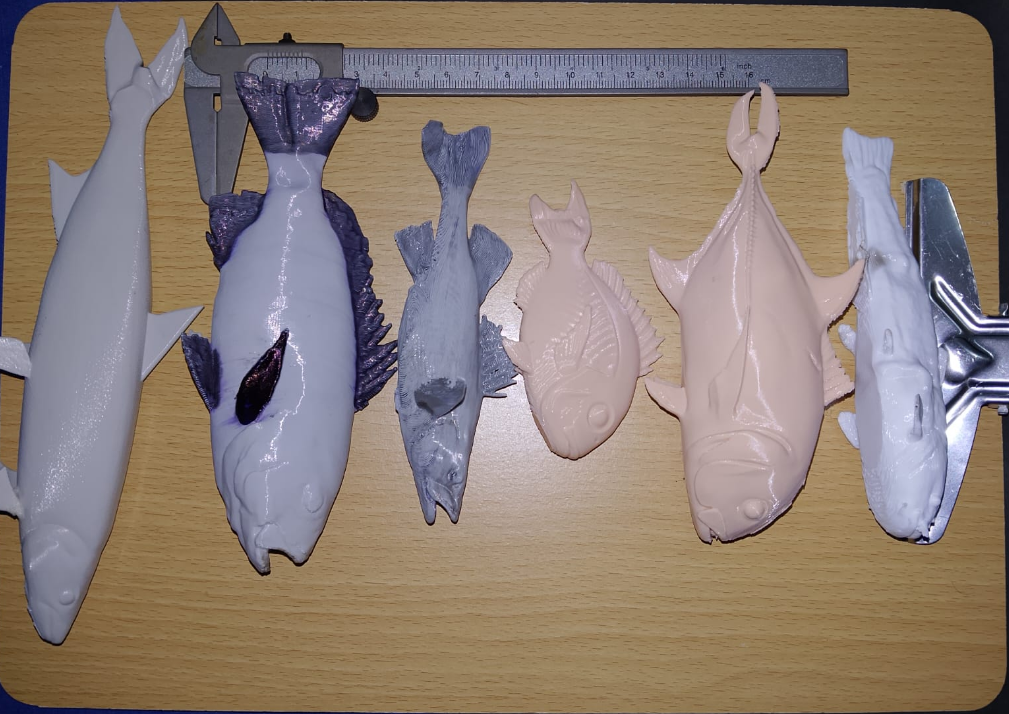
\includegraphics[width=0.8\textwidth]{fig3_1_replicas.png}
\caption[Réplicas de peces impresas en PLA utilizadas en el experimento]{Réplicas de peces impresas en PLA utilizadas en el experimento. Fuente: elaboración propia.}
\label{fig:3-1}
\end{figure}

\begin{table}[htbp]
\centering\footnotesize
\caption{Réplicas y referencias físicas medidas con calibre.}
\label{tab:replicas}
\begin{tabular}{@{}lp{1.6cm}p{1.5cm}p{1.6cm}p{1.5cm}@{}}
\toprule
Réplica & LT media (mm) & Desv. LT (mm) & PC media (mm) & Desv. PC (mm) \\
\midrule
R1 & 158,7 & 1,5 & 45,0 & 0,0 \\
R2 & 134,3 & 2,9 & 27,3 & 0,6 \\
R3 & 91,7 & 0,6 & 40,3 & 0,6 \\
R4 & 142,7 & 2,9 & 42,7 & 0,6 \\
R5 & 137,3 & 0,6 & 25,7 & 0,6 \\
R6 & 209,7 & 0,6 & 35,3 & 0,6 \\
\bottomrule
\end{tabular}
\end{table}

Tomamos cada medida de referencia tres veces con un calibre analógico con nonio (Figura~\ref{fig:H-2}) y registramos las lecturas al milímetro. La media es la referencia; la desviación estándar muestral entre lecturas indica cuán repetible es (Tabla~\ref{tab:replicas}). La mayor desviación fue de 2,9~mm, en la LT de R2 y R4; en PC no pasó de 0,6~mm. Estas desviaciones son menores que el MAE de A y \Aprime, pero del mismo orden o mayores que el de B y C (1,08 y 1,22~mm en LT; 0,38 y 0,56~mm en PC; Tabla~\ref{tab:agregados}). Dicho de otro modo: el error de B y C ya es comparable con la incertidumbre de la propia regla con la que los juzgamos.

Ubicamos cada réplica con su plano de simetría a cuatro distancias nominales de la cara interna del vidrio: 5, 11, 17 y 23~cm. Elegimos esas posiciones por los límites físicos de la pecera y por la zona en la que la imagen seguía bien enfocada. En cada combinación de réplica y distancia tomamos tres fotografías técnicas. Entre repeticiones no movimos ni la cámara ni la pecera: volvíamos a colocar la réplica en su posición y disparábamos de nuevo. Fotografiamos réplica por réplica, completando sus cuatro distancias y sus repeticiones antes de pasar a la siguiente.

No variamos de forma planificada la posición de la réplica dentro del encuadre, así que el diseño solo cambia la profundidad. El experimento produjo $6 \times 4 \times 3 = 72$ imágenes originales. Las repeticiones de una misma réplica son repeticiones técnicas y no réplicas independientes; por eso el número de unidades experimentales es $n = 6$ y el de combinaciones réplica--profundidad, 24.

Incluimos las capturas en las que la réplica se veía completa y bien enfocada. Las que no cumplían estas condiciones las descartamos y anotamos el motivo en la tabla maestra. La muestra refleja las réplicas disponibles y el tiempo destinado al experimento; por eso leemos los resultados como una evaluación experimental del montaje, no como una generalización a todos los peces.

\section{Montaje e instrumentos de recolección de datos}
\label{sec:montaje}

El ensayo se hizo en una pecera de aproximadamente $30 \times 30 \times 30$~cm, de vidrio \emph{float} de 4,0~mm de espesor, medido con calibre, llena de agua clara de la canilla. Para el modelo óptico adoptamos $\mu_a = 1{,}000$, $\mu_g = 1{,}500$ y $\mu_w = 1{,}333$, valores tabulados y no medidos en nuestra agua. La Figura~\ref{fig:3-esquema} muestra el esquema acotado del montaje, y el Anexo~\ref{anx:montaje} reúne fotografías de la pecera y de los instrumentos.

\begin{figure}[htbp]
\centering
\begin{tikzpicture}[scale=0.34,>=Stealth,font=\scriptsize]
  % pecera (vista superior): vidrio frontal en x=0, interior de 0 a 30 cm
  \fill[cyan!8] (0,0) rectangle (30,30);
  \draw[gray!60!black,line width=1.5pt] (0,0) rectangle (30,30);
  \node[gray!60!black,font=\scriptsize] at (15,28.3) {pecera $30 \times 30 \times 30$ cm (vista superior)};
  \draw[line width=2.5pt,gray!70!black] (0,0) -- (0,30);
  \node[rotate=90,gray!70!black,font=\scriptsize] at (-1.6,22.5) {vidrio frontal, $t_g = 4$ mm};
  % cámara (distancia comprimida, con corte)
  \node[draw,fill=white,minimum width=1.0cm,minimum height=0.7cm] (cam) at (-9.5,15) {};
  \fill (-8.6,15) circle (2pt);
  \node[above=2pt,font=\scriptsize,align=center] at (cam.north) {cámara\\(Realme C71)};
  \draw[->,thick] (-8.6,15) -- (0,15);
  \draw[thick] (-5.2,14.2) -- (-4.6,15.8); \draw[thick] (-4.8,14.2) -- (-4.2,15.8);
  \draw[<->] (-8.6,12.3) -- (0,12.3) node[midway,below,font=\scriptsize,align=center] {$d = 230$ mm\\(no a escala)};
  % ArUco 1 en el vidrio
  \fill[metA] (0.3,19) rectangle (1.1,22);
  \node[metA,right,font=\scriptsize,align=left] at (1.3,20.5) {ArUco id 1 (A),\\fijo en el vidrio};
  % riel
  \draw[very thick,black!60] (2,15) -- (28,15);
  \node[black!60,below,font=\scriptsize] at (25.5,14.6) {riel con carrito};
  \foreach \p/\lab in {5/5,11/11,17/17,23/23}{
    \draw[metC,very thick] (\p,13.4) -- (\p,16.6);
    \node[metC,above,font=\scriptsize] at (\p,16.7) {\lab\,cm};
  }
  % réplica en 11 cm
  \draw[metC,line width=2.5pt] (11,9) -- (11,21);
  \node[metC,left,align=right,font=\scriptsize] at (10.5,10.2) {réplica\\(plano de simetría)};
  % ArUco 2 coplanar
  \fill[metAp] (10.6,6.2) rectangle (11.4,8.6);
  \node[metAp,right,font=\scriptsize,align=left] at (11.7,7.4) {ArUco id 0 (\Aprime),\\en el carrito};
  % lámpara
  \node[draw,circle,fill=yellow!40,minimum size=0.5cm] at (15,32.5) {};
  \node[above,font=\scriptsize] at (15,33.2) {foco 12 W (techo)};
  \draw[dashed] (0,15) -- (30,15);
  \draw[<->,thick] (0.2,3.5) -- (11,3.5) node[midway,below,font=\scriptsize] {$z$ (desde la cara interna del vidrio)};
\end{tikzpicture}
\caption[Esquema acotado del montaje experimental]{Esquema acotado del montaje experimental en vista superior: cámara a $d = 230$~mm del vidrio frontal de 4~mm, marcador ArUco fijo en el vidrio (ruta A), riel con carrito y cuatro posiciones nominales (5, 11, 17 y 23~cm), marcador coplanar en el carrito (ruta \Aprime) e iluminación cenital fija. No está a escala. Fuente: elaboración propia.}
\label{fig:3-esquema}
\end{figure}

La cámara fue la de un teléfono común, un Realme C71 RMX5303 Dual. Guardamos las capturas en JPG a $4096 \times 3072$ píxeles, con la configuración bloqueada durante todo el ensayo: ISO 640, velocidad de obturación 1/25~s, enfoque 0,76 y balance de blancos 5600~K. Medimos con una regla 230~mm entre el frente de la lente y el vidrio, y usamos esa distancia como aproximación de la distancia entre el centro de proyección y la primera interfaz. En la cámara de un teléfono, la diferencia entre el frente de la lente y el centro de proyección es de pocos milímetros; su efecto sobre C lo cuantificamos en la Sección~\ref{sec:sensibilidad} con un análisis de sensibilidad a $d$. Comprobamos con una escuadra que el eje de la cámara fuera aproximadamente perpendicular al vidrio.

La iluminación fue siempre la misma: un foco de bajo consumo de 12~W en el techo de la habitación, con la pecera debajo. La réplica iba montada en un carrito que se desliza sobre un riel, ambos impresos en PLA. Ese soporte permitió repetir las posiciones de profundidad y mantener la réplica con una orientación parecida entre capturas. La Tabla~\ref{tab:posiciones} relaciona la posición nominal de cada captura con la lectura del riel y con el origen de coordenadas que usa B. El cero del riel coincide con la posición de 5~cm, donde calibramos B; por eso B recibió como posición del plano de medición la lectura del riel, $z_{\mathrm{riel}} = z - 50$~mm, mientras que C usó la distancia absoluta $z$ a la cara interna del vidrio.

\begin{table}[htbp]
\centering\footnotesize
\caption{Correspondencia entre la posición nominal de la réplica y la lectura del riel.}
\label{tab:posiciones}
\begin{tabular}{@{}p{2.8cm}p{3.4cm}p{2.6cm}p{3.4cm}@{}}
\toprule
Posición nominal (cm al vidrio) & Separación de la zona de calibración de B (cm) & Lectura del riel (mm) & Desplazamiento al plano de simetría (mm) \\
\midrule
5  & 0  & 0   & 10, compensado \\
11 & 6  & 60  & 10, compensado \\
17 & 12 & 120 & 10, compensado \\
23 & 18 & 180 & 10, compensado \\
\bottomrule
\end{tabular}

\smallskip
\begin{minipage}{0.9\textwidth}\footnotesize
\emph{Nota.} El plano de simetría de la réplica quedaba 10~mm corrido respecto del apoyo del carrito. Compensamos ese desplazamiento físicamente en el montaje, corriendo el carrito 10~mm para que el plano de simetría quedara en la posición nominal; por eso el procesamiento no aplicó ningún desplazamiento adicional, y el registro de datos consigna un desplazamiento de réplica de 0~mm.
\end{minipage}
\end{table}

Usamos dos marcadores ArUco del diccionario \texttt{4X4\_50}, con los identificadores 0 y 1. El id~1, el de la ruta A, quedó fijo en el vidrio. El id~0, el de \Aprime, fue en una base común con la réplica. Para acercarlo al plano de simetría lo montamos sobre un separador de isopor del largo equivalente al eje de simetría, sujeto con cinta impermeable de doble faz. La réplica se fijó a la base con el alambre que pasa por sus orificios. Medimos ambos marcadores con calibre: cada uno ocupa un cuadrado de 70~mm de lado, margen blanco incluido, y el cuadrado negro mide 60~mm. Como el detector ubica las esquinas en el borde exterior del cuadrado negro, el lado que cuenta es ese, y coincide con el valor $L_m = 60{,}0$~mm configurado en el procesamiento. La Figura~\ref{fig:3-2} muestra una réplica con su marcador coplanar dentro de la pecera.

\begin{figure}[htbp]
\centering
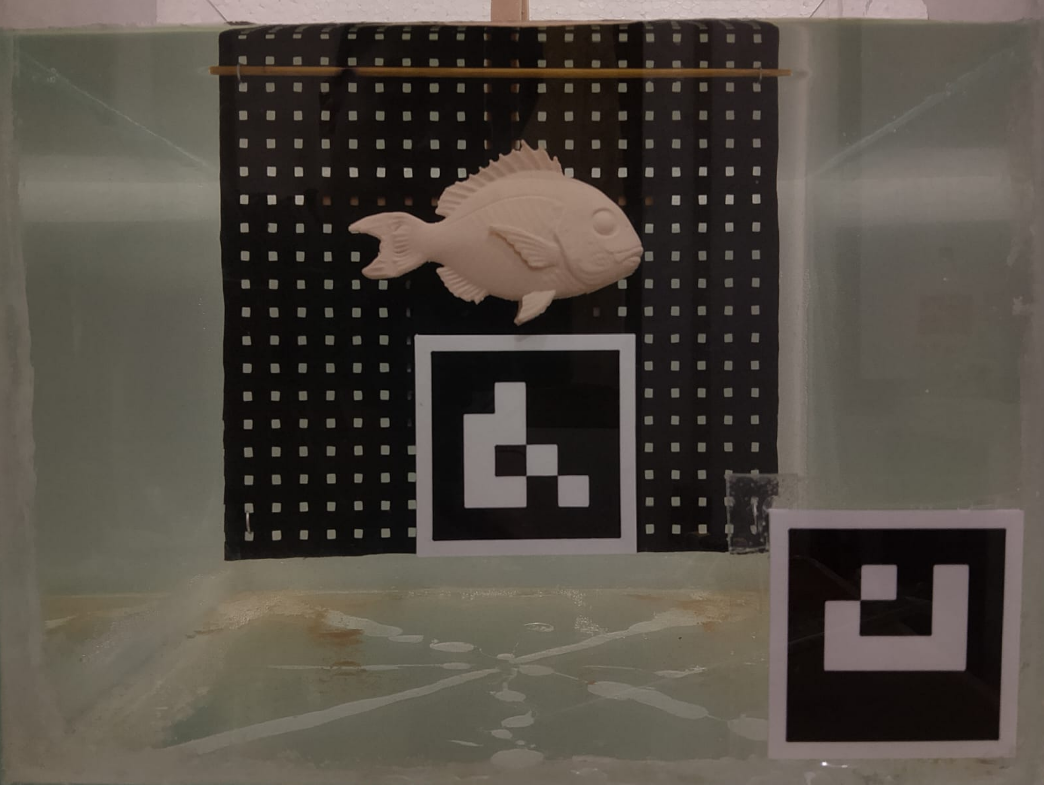
\includegraphics[width=0.75\textwidth]{fig3_2_montaje_replica.png}
\caption[Montaje de una réplica junto con el marcador ArUco coplanar]{Montaje de una réplica junto con el marcador ArUco coplanar. Fuente: elaboración propia.}
\label{fig:3-2}
\end{figure}

Para calibrar usamos un damero de $5 \times 5$ cuadros ($4 \times 4$ esquinas interiores) con cuadros de 20~mm. La calibración de B se hizo en la posición más cercana al vidrio, la de 5~cm. La separación de cada captura respecto de esa zona es la diferencia absoluta entre su distancia al vidrio y la distancia de calibración. La Figura~\ref{fig:3-3} muestra el damero y el marcador durante la preparación de la calibración.

\begin{figure}[htbp]
\centering
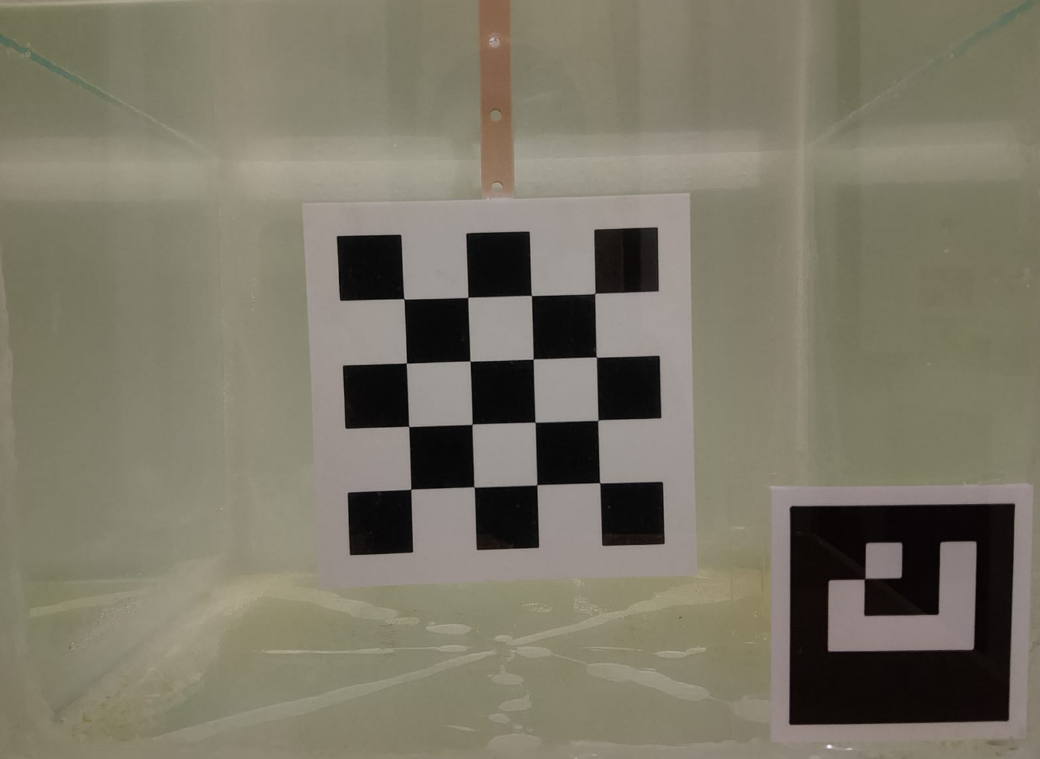
\includegraphics[width=0.75\textwidth]{fig3_3_damero.png}
\caption[Damero y marcador ArUco colocados dentro de la pecera]{Damero y marcador ArUco colocados dentro de la pecera. Fuente: elaboración propia.}
\label{fig:3-3}
\end{figure}

La Tabla~\ref{tab:puerto} reúne los parámetros físicos del puerto plano que usa C. Son, en la práctica, la ficha técnica del instrumento, y se conservan en el archivo de configuración reproducido en el Anexo~\ref{anx:flatport}.

\begin{table}[htbp]
\centering\footnotesize
\caption{Parámetros del puerto plano utilizados por la ruta C.}
\label{tab:puerto}
\begin{tabular}{@{}p{3.6cm}p{2.6cm}p{1.2cm}p{5.4cm}@{}}
\toprule
Parámetro & Valor & Unidad & Cómo se obtuvo \\
\midrule
Normal del puerto $\mathbf{n}_\pi$ & $(0, 0, 1)$ & --- & Supuesta perpendicular; comprobada con escuadra \\
Distancia cámara--vidrio $d$ & 230 & mm & Regla, desde el frente de la lente \\
Espesor del vidrio $t_g$ & 4,0 & mm & Calibre \\
Índice del aire $\mu_a$ & 1,000 & --- & Valor tabulado \\
Índice del vidrio $\mu_g$ & 1,500 & --- & Valor tabulado (vidrio \emph{float}) \\
Índice del agua $\mu_w$ & 1,333 & --- & Valor tabulado (agua dulce, 22~\si{\celsius}) \\
Condiciones del agua & 22~\si{\celsius}; salinidad 0; 0~dbar & --- & Registradas en la configuración \\
\bottomrule
\end{tabular}
\end{table}

Para ubicar el plano de medición de B observamos el damero en dos posiciones del riel (0 y 180~mm). La Tabla~\ref{tab:riel} resume los valores principales y el Anexo~\ref{anx:riel} reproduce el archivo completo. El residuo del ajuste de la dirección del riel ($1{,}62 \times 10^{-13}$~mm) es el de una recta que pasa por dos puntos: un residuo numérico, no una medida de precisión física. Los indicadores que sí informan sobre la calidad quedaron dentro de los umbrales configurados: el error de reproyección fue de 0,270~px y la dispersión de la normal, de $0{,}337^{\circ}$ (umbrales de 1,0~px y $1{,}0^{\circ}$), y el error relativo de escala, de 0,813~\%, quedó por debajo del umbral de 5~\%.

\begin{table}[htbp]
\centering\small
\caption{Referencia geométrica del riel utilizada por la ruta B.}
\label{tab:riel}
\begin{tabular}{@{}p{6cm}p{7cm}@{}}
\toprule
Campo & Valor \\
\midrule
Plano de referencia $z_{\mathrm{ref}}$ & 0,0~mm (posición nominal de 5~cm) \\
Posiciones del riel utilizadas & 0,0 y 180,0~mm \\
Error de reproyección (umbral) & 0,270~px (1,0~px) \\
Dispersión de la normal (umbral) & $0{,}337^{\circ}$ ($1{,}0^{\circ}$) \\
Error relativo de escala (umbral) & 0,813~\% (5~\%) \\
Supuesto & Planos de las réplicas paralelos al tablero \\
\bottomrule
\end{tabular}
\end{table}

\section{Software utilizado}
\label{sec:software}

Procesamos las imágenes con Fishmeter, una aplicación propia escrita en Python 3.12. El código fuente y la documentación de uso están en el repositorio público \url{\RepoURL}, etiqueta \texttt{\RepoTag}. La aplicación usa OpenCV 5.0.0 para detectar marcadores, calibrar y aplicar transformaciones geométricas; NumPy 2.5.3 para el cálculo vectorial; PyYAML 6.0.3 para los archivos de configuración; y Tkinter, de la biblioteca estándar, para la interfaz gráfica.
\\
El módulo refractivo (\texttt{refractive\_port.py} y \texttt{snells\_law.py}) implementa las ecuaciones~\eqref{eq:va} a~\eqref{eq:rayo} e incluye pruebas unitarias de sanidad. Con $\mu_g = \mu_w = 1$ y $t_g = 0$, es decir, sin vidrio ni agua, reproduce la cámara pinhole; y un rayo que viaja sobre el eje óptico no se desvía. Las pruebas de integración verifican que los cuatro métodos reciban las mismas coordenadas y que cada imagen produzca un registro trazable.

Desde la interfaz se carga la fotografía, se detectan los marcadores, se cargan o se marcan a mano los puntos anatómicos, se ejecutan los cuatro métodos y se exportan los resultados. Los clics sobre el visor se convierten a coordenadas de la imagen original antes de guardarlos o procesarlos. La Figura~\ref{fig:3-4} muestra la pantalla de marcado y comparación.

\begin{figure}[htbp]
\centering
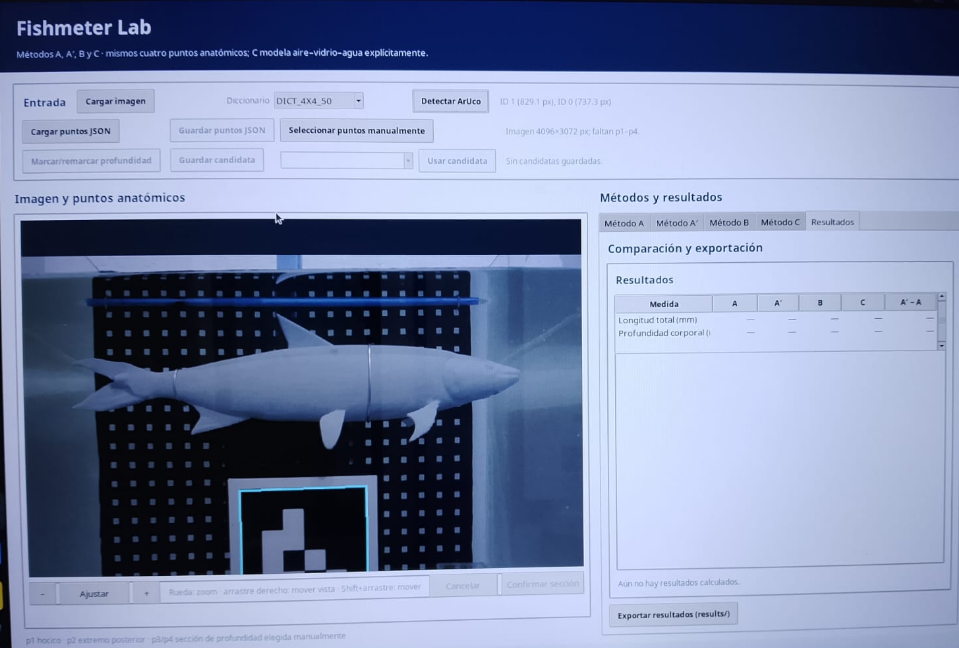
\includegraphics[width=0.8\textwidth]{fig3_4_interfaz.png}
\caption[Interfaz de Fishmeter para la marcación y comparación de métodos]{Interfaz de Fishmeter para la marcación y comparación de métodos. Fuente: Fishmeter.}
\label{fig:3-4}
\end{figure}

\section{Medidas físicas, puntos anatómicos y variables}
\label{sec:medidas}

Para cada réplica conservamos las medidas físicas de referencia de la longitud total y de la profundidad corporal (Tabla~\ref{tab:replicas}). La referencia y la imagen siguieron la misma convención anatómica, la de la Sección~\ref{sec:puntos-def}. La longitud total va desde el extremo anterior del hocico ($\mathbf{p}_1$) hasta el punto más posterior de la aleta caudal sobre el eje longitudinal ($\mathbf{p}_2$); si la cola tiene dos lóbulos, $\mathbf{p}_2$ es el extremo del lóbulo más largo. La profundidad corporal va del perfil dorsal ($\mathbf{p}_3$) al perfil ventral ($\mathbf{p}_4$) en una misma sección transversal, sin incluir las aletas.

Marcamos los cuatro puntos a mano sobre la imagen original e indicamos de forma explícita el eje longitudinal de la réplica, que usamos para proyectar las medidas. No hubo segmentación automática ni puntos distintos para cada método. La Figura~\ref{fig:3-5} resume dónde van los cuatro puntos y qué miden, y la Figura~\ref{fig:3-6} muestra los instrumentos con los que obtuvimos las dimensiones físicas de referencia.

\begin{figure}[htbp]
\centering
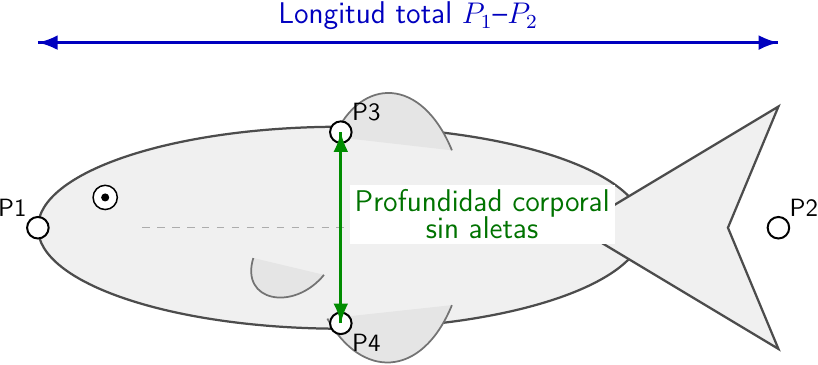
\includegraphics[width=0.7\textwidth]{fig3_5_puntos.png}
\caption[Puntos anatómicos empleados para la longitud total y la profundidad corporal]{Puntos anatómicos empleados para la longitud total y la profundidad corporal. Fuente: elaboración propia.}
\label{fig:3-5}
\end{figure}

\begin{figure}[htbp]
\centering
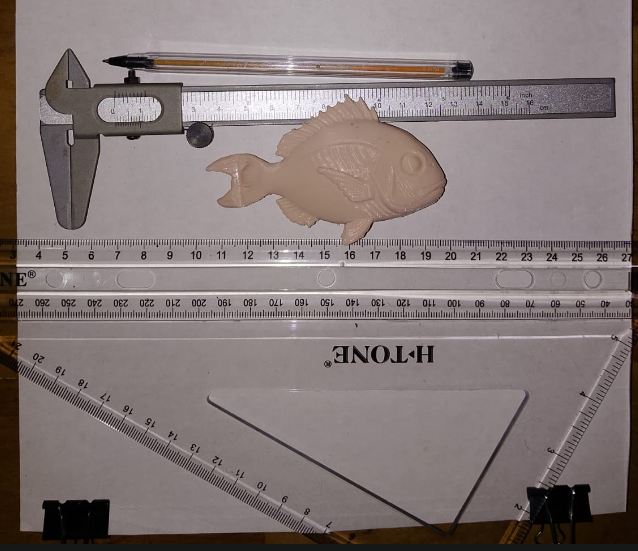
\includegraphics[width=0.6\textwidth]{fig3_6_instrumentos.png}
\caption[Instrumentos y disposición utilizados para medir físicamente una réplica]{Instrumentos y disposición utilizados para medir físicamente una réplica. Fuente: elaboración propia.}
\label{fig:3-6}
\end{figure}

Si $\mathbf{u}$ es el vector unitario del eje longitudinal y $\mathbf{n} = (-u_y, u_x)$ su normal, calculamos las medidas en el plano métrico como
\begin{equation}
\mathrm{LT} = \lvert (\mathbf{q}_2 - \mathbf{q}_1)\cdot\mathbf{u} \rvert, \qquad
\mathrm{PC} = \lvert (\mathbf{q}_4 - \mathbf{q}_3)\cdot\mathbf{n} \rvert,
\label{eq:medidas}
\end{equation}
donde $\mathbf{q}_i$ son los puntos anatómicos ya convertidos a milímetros por cada ruta. En la práctica, LT es la proyección del segmento $\mathbf{p}_1$--$\mathbf{p}_2$ sobre el eje longitudinal; si los puntos están sobre el eje, coincide con la distancia en línea recta, que es lo que mide el calibre. Una aclaración sobre los datos: en los registros del experimento, los rótulos $\mathbf{p}_1$ y $\mathbf{p}_2$ quedaron invertidos respecto de esta definición, de modo que $\mathbf{p}_1$ se marcó en el extremo caudal y $\mathbf{p}_2$ en el hocico. Como LT se calcula con el valor absoluto de la proyección (ecuación~\ref{eq:medidas}), el orden de los puntos no cambia el resultado. Solo aceptamos la profundidad corporal cuando la sección marcada era lo bastante perpendicular al eje; la aplicación guardó ese desvío como diagnóstico y permitió descartar una profundidad no válida.

La Tabla~\ref{tab:operacionalizacion} define cada variable en términos conceptuales y operacionales, y separa lo que variamos, lo que medimos y lo que mantuvimos fijo.

\begin{table}[htbp]
\centering\footnotesize
\caption{Operacionalización de las variables.}
\label{tab:operacionalizacion}
\begin{tabularx}{\textwidth}{@{}p{2.3cm} p{1.3cm} X X p{1.2cm}@{}}
\toprule
Variable & Tipo & Definición conceptual & Definición operacional & Unidad \\
\midrule
\multicolumn{5}{@{}l}{\emph{Factores variados}}\\
Método & Nominal & Ruta de conversión píxel--milímetro & A, \Aprime, B o C aplicados a los mismos puntos (Sección~\ref{sec:metodos}) & --- \\
Distancia al vidrio & Nominal & Profundidad $z$ del plano de simetría de la réplica & Posición del carrito: 5, 11, 17 o 23~cm; separación de la zona de B: 0, 6, 12 o 18~cm & cm \\
Rango de $z$ & Nominal & Conocimiento disponible sobre la profundidad & Toda la pecera (0--30~cm); $\pm 3$~cm; $\pm 1$~cm & cm \\
\multicolumn{5}{@{}l}{\emph{Resultados medidos}}\\
LT y PC estimadas & Razón & Longitud total y profundidad corporal de la réplica & Salida de Fishmeter por método, ecuación~\eqref{eq:medidas} & mm \\
LT y PC de referencia & Razón & Dimensión física de la réplica & Media de tres lecturas con calibre analógico, registradas al milímetro & mm \\
Error con signo, EA, EPA & Razón & Diferencia entre estimación y referencia & Ecuaciones~\eqref{eq:errores} & mm, mm, \% \\
Ancho relativo de $\IL$ & Razón & Extensión del intervalo por profundidad desconocida & $(\max_z L - \min_z L)/\mathrm{LT}_{\mathrm{ref}}$ & \% \\
Cobertura de $\IL$ & Razón & Fracción de capturas cuya referencia cae en $\IL$ & Conteo sobre las capturas disponibles & --- \\
\multicolumn{5}{@{}l}{\emph{Condiciones fijas}}\\
Cámara, pecera, agua, luz, marcadores, soporte, operador & --- & Condiciones del montaje & Registradas en las Secciones~\ref{sec:montaje} y~\ref{sec:procedimiento} & --- \\
\bottomrule
\end{tabularx}
\end{table}

\section{Métodos de conversión métrica}
\label{sec:metodos}

Los cuatro métodos reciben la misma imagen, los mismos cuatro puntos y el mismo eje. Lo único que cambia es la transformación que convierte píxeles en milímetros.

\begin{description}
  \item[Método A.] Usa el ArUco fijo en el vidrio. Con el lado físico $L_m$ del marcador y el promedio $\bar{p}$ de las longitudes en píxeles de sus cuatro lados (ecuación~\ref{eq:lado}), la escala implementada es
  \begin{equation}
    k = \frac{L_m}{\bar{p}}, \qquad \bar{p} = \frac{1}{4}\sum_{i=1}^{4} p_i,
    \label{eq:escala-impl}
  \end{equation}
  que difiere de la ecuación~\eqref{eq:escala-monkman} solo en el orden en que se promedia; para marcadores bien detectados, ambas coinciden hasta la tercera cifra. Cada punto se transforma como $\mathbf{q}_i = k\,\mathbf{p}_i$ y las medidas salen de la ecuación~\eqref{eq:medidas}. Es la línea de base: no corrige la diferencia de profundidad entre el vidrio y la réplica.
  \item[Método \Aprime.] Usa el ArUco montado aproximadamente en el plano de simetría de la réplica. Las cuatro esquinas del marcador en píxeles y sus coordenadas métricas $(0,0)$, $(L_m,0)$, $(L_m,L_m)$ y $(0,L_m)$ definen una homografía $\mathbf{H}$ de $3 \times 3$. Cada punto anatómico se transforma como $\tilde{\mathbf{q}}_i = \mathbf{H}\,\tilde{\mathbf{p}}_i$, en milímetros sobre el plano del marcador; el eje longitudinal se transforma igual, y las medidas salen de la ecuación~\eqref{eq:medidas}. La homografía corrige la perspectiva dentro del plano del marcador, pero no la diferencia de escala de los puntos que quedan fuera de él.
  \item[Método B.] Usa la calibración de cámara hecha con el damero sumergido y un modelo pinhole efectivo (perfil \texttt{B-effective}, Anexo~\ref{anx:calibraciones}). Los píxeles se convierten en rayos con $\mathbf{K}_{\mathrm{agua}}$ y los coeficientes de distorsión efectivos (ecuaciones~\ref{eq:pinhole} y~\ref{eq:distorsion}, invertidas), y esos rayos se intersecan con el plano $\pi_z$, paralelo al tablero de calibración y ubicado en la lectura del riel de cada captura, que ya corresponde al plano de simetría de la réplica (Tabla~\ref{tab:posiciones}). Como la calibración se fijó en la posición más cercana al vidrio, B representa de forma empírica el comportamiento óptico de esa zona. LT y PC se calculan en el espacio métrico tridimensional.
  \item[Método C.] Usa la calibración de cámara hecha en aire (perfil \texttt{C-air}) y el modelo de puerto plano de la Sección~\ref{sec:puerto-plano}. Para cada punto corregimos la distorsión de la lente, obtenemos el rayo en el aire (ecuación~\ref{eq:va}), aplicamos las dos refracciones (ecuaciones~\ref{eq:q1} a~\ref{eq:vw}) con los parámetros de la Tabla~\ref{tab:puerto} e intersecamos el rayo en el agua (ecuación~\ref{eq:rayo}) con el plano de la réplica, definido en el marco de la cámara física. Para el caso de profundidad desconocida repetimos el cálculo sobre la grilla de profundidades físicamente admisibles y lo expresamos como el intervalo geométrico de la ecuación~\eqref{eq:IL}.
\end{description}

Teníamos prevista una prueba complementaria con una barra patrón sumergida, pensada para separar un posible error de implementación del error de marcado. No la hicimos como validación separada; solo hubo una comprobación preliminar con la réplica R1 (de unos 160~mm de largo), durante las pruebas de comienzos de septiembre de 2026 (Sección~\ref{sec:delimitacion}). La validación métrica de las cuatro rutas es, entonces, la comparación directa con las longitudes y profundidades medidas con calibre en las seis réplicas y las cuatro posiciones (Capítulo~\ref{cap:resultados}). A lo largo del documento distinguimos la «comprobación instrumental con patrón» (barra sumergida, no realizada) de la «validación externa» (otras cámaras, montajes o condiciones, fuera del alcance).

\subsection{Implementación en Fishmeter}
\label{sec:implementacion}

En Fishmeter, los cuatro métodos comparten el principio y el final del cálculo. Todos parten de los mismos cuatro puntos y del mismo eje longitudinal marcados en la imagen; en todas las capturas, ese eje se indicó como la dirección horizontal de la imagen, $(1, 0)$. Todos terminan, también, en la misma operación: proyectar los segmentos $\mathbf{p}_1$--$\mathbf{p}_2$ y $\mathbf{p}_3$--$\mathbf{p}_4$ sobre los ejes anatómicos. Lo que cambia es el camino que lleva los píxeles a un espacio métrico. A y \Aprime{} llegan a un plano bidimensional en milímetros; B y C, a un plano ubicado en el espacio tridimensional de la cámara. La Tabla~\ref{tab:recorridos} resume ese camino con los nombres de las funciones del repositorio (Sección~\ref{sec:software}).

\begin{table}[htbp]
\centering\footnotesize
\caption{Recorrido de cada método en Fishmeter, desde los píxeles hasta la medición.}
\label{tab:recorridos}
\begin{tabularx}{\textwidth}{@{}p{1.1cm} >{\raggedright\arraybackslash}X >{\raggedright\arraybackslash}p{1.9cm} >{\raggedright\arraybackslash\scriptsize\ttfamily}p{5.4cm}@{}}
\toprule
Método & Conversión de los puntos & Espacio de medición & \normalfont\footnotesize Funciones principales \\
\midrule
A & Escala uniforme $k$ tomada del ArUco fijo en el vidrio & Plano 2D & measure\_a $\rightarrow$ measure\_direct $\rightarrow$ scale\_points $\rightarrow$ measure\_projected\_morphometry \\
\Aprime & Homografía $\mathbf{H}$ entre las esquinas del ArUco coplanar y un cuadrado de lado $L_m$ & Plano 2D & measure\_a\_prime $\rightarrow$ measure\_direct $\rightarrow$ marker\_plane\_homography $\rightarrow$ transform\_points\_homography $\rightarrow$ measure\_projected\_morphometry \\
B & Rayo del modelo pinhole efectivo intersecado con el plano $\pi_z$ ubicado con el riel & Plano en el espacio 3D & measure\_b $\rightarrow$ intersect\_image\_points\_with\_plane $\rightarrow$ intersect\_ray\_plane $\rightarrow$ measure\_projected\_morphometry\_3d \\
C & Rayo en aire refractado en las interfaces aire--vidrio y vidrio--agua, e intersecado con el plano de la réplica & Plano en el espacio 3D & measure\_c $\rightarrow$ \_trace\_to\_plane $\rightarrow$ trace\_refracted\_ray $\rightarrow$ intersect\_ray\_line\_plane $\rightarrow$ measure\_projected\_morphometry\_3d \\
\bottomrule
\end{tabularx}
\end{table}

\paragraph{Método A.} La función \texttt{measure\_direct} calcula el factor $k$ de la ecuación~\eqref{eq:escala-impl} y multiplica por él las coordenadas de los cuatro puntos, $\mathbf{q}_i = k\,\mathbf{p}_i$. Como una escala uniforme no cambia las direcciones, el eje marcado en la imagen sirve sin modificaciones en el plano métrico. Cada resultado de A sale con una advertencia automática: la escala viene del plano del vidrio y no corrige la separación entre planos, la perspectiva ni la refracción.

\paragraph{Método \Aprime.} La misma función calcula con OpenCV la homografía que lleva las cuatro esquinas detectadas del marcador al cuadrado métrico de lado $L_m$, y la aplica a los cuatro puntos. Una homografía no conserva las direcciones de la imagen, así que el eje se transforma como una recta: Fishmeter toma $\mathbf{p}_1$ y un segundo punto desplazado sobre el eje, transforma ambos y usa como eje métrico la dirección que los une. Lo mismo se hace en B y en C.

\paragraph{Método B.} Primero se ubica el plano de medición. El plano de referencia que guarda la calibración del riel, con un punto $\mathbf{P}_{\mathrm{ref}}$ y una normal $\mathbf{s}$, se traslada a lo largo de la dirección del riel la diferencia entre la lectura de la captura y la de calibración, $z_{\mathrm{riel}} - z_{\mathrm{ref}}$ (Tablas~\ref{tab:posiciones} y~\ref{tab:riel}); así se obtiene un punto $\mathbf{P}_0$ del plano $\pi_z$. La normal no cambia, porque suponemos que los planos de las réplicas son paralelos al tablero. Después, cada punto se corrige de distorsión con $\mathbf{K}_{\mathrm{agua}}$ y los coeficientes del perfil \texttt{B-effective}, se convierte en un rayo $\mathbf{r} = (x, y, 1)^{\mathsf{T}}$ que sale del centro de la cámara y se interseca con el plano:
\begin{equation}
\mathbf{P} = \lambda\,\mathbf{r}, \qquad \lambda = \frac{\mathbf{s}\cdot\mathbf{P}_0}{\mathbf{s}\cdot\mathbf{r}} .
\label{eq:interseccion-b}
\end{equation}
La refracción no aparece en ningún paso: queda absorbida, de forma empírica, en la calibración hecha bajo el agua.

\paragraph{Método C.} Cada punto se corrige de distorsión con la calibración en aire (perfil \texttt{C-air}) y da la dirección $\mathbf{v}_a$ de la ecuación~\eqref{eq:va}. La función \texttt{trace\_refracted\_ray} sigue ese rayo hasta la cara exterior del vidrio ($\mathbf{q}_1$), lo refracta con la ley de Snell vectorial ($\mathbf{v}_g$), lo lleva hasta la cara interior ($\mathbf{q}_2$) y lo vuelve a refractar al entrar en el agua ($\mathbf{v}_w$); son las ecuaciones~\eqref{eq:q1} a~\eqref{eq:vw}, en ese orden. En cada interfaz comprueba que el punto calculado quede sobre el plano del vidrio, con una tolerancia de $10^{-6}$~mm. El rayo en el agua (ecuación~\ref{eq:rayo}) se interseca después con el plano de la réplica, que en C es paralelo al vidrio ($\mathbf{s} = \mathbf{n}_\pi$) y contiene el punto $\mathbf{P}_0$ ubicado a $d + t_g + z$ del centro de la cámara sobre esa normal:
\begin{equation}
\mathbf{P} = \mathbf{q}_2 + \lambda\,\mathbf{v}_w, \qquad \lambda = \frac{\mathbf{s}\cdot(\mathbf{P}_0 - \mathbf{q}_2)}{\mathbf{s}\cdot\mathbf{v}_w} .
\label{eq:interseccion-c}
\end{equation}
Los dos puntos que definen el eje se trazan de la misma forma, de modo que los puntos anatómicos y el eje quedan en el mismo sistema de coordenadas.

\paragraph{Medición final.} A y \Aprime{} aplican directamente la ecuación~\eqref{eq:medidas}. En B y C, el eje transformado $\mathbf{a}$ se proyecta primero sobre el plano de medición, para quitarle cualquier componente fuera de él, y la dirección dorsoventral se obtiene con el producto vectorial:
\begin{equation}
\mathbf{u} = \frac{\mathbf{a} - (\mathbf{a}\cdot\mathbf{s})\,\mathbf{s}}{\lVert \mathbf{a} - (\mathbf{a}\cdot\mathbf{s})\,\mathbf{s} \rVert}, \qquad
\mathbf{n} = \mathbf{s} \times \mathbf{u} .
\label{eq:ejes-3d}
\end{equation}
Con esos ejes, LT y PC salen de la misma ecuación~\eqref{eq:medidas}, con los puntos tridimensionales $\mathbf{P}_i$ en lugar de $\mathbf{q}_i$. En los cuatro métodos, la profundidad corporal se valida con el ángulo de la sección,
\begin{equation}
\theta = \arctan\frac{\lvert (\mathbf{q}_4 - \mathbf{q}_3)\cdot\mathbf{u} \rvert}{\lvert (\mathbf{q}_4 - \mathbf{q}_3)\cdot\mathbf{n} \rvert},
\label{eq:angulo-seccion}
\end{equation}
que mide cuánto se aparta el segmento $\mathbf{p}_3$--$\mathbf{p}_4$ de la perpendicular al eje. Si $\theta$ supera $5^{\circ}$, Fishmeter no informa la PC y deja una advertencia; en nuestros datos ningún registro superó ese umbral. Las distancias euclidianas $\lVert \mathbf{q}_2 - \mathbf{q}_1 \rVert$ y $\lVert \mathbf{q}_4 - \mathbf{q}_3 \rVert$ se guardan con cada resultado, pero solo como diagnóstico.

\section{Procedimiento por imagen y trazabilidad}
\label{sec:procedimiento}

Las 72 imágenes siguieron exactamente la misma secuencia, la de la Figura~\ref{fig:3-flujo}:

\begin{enumerate}
  \item identificar la réplica, la distancia y la repetición, y conservar la imagen JPG original;
  \item verificar visibilidad y enfoque;
  \item marcar manualmente $\mathbf{p}_1$, $\mathbf{p}_2$, $\mathbf{p}_3$ y $\mathbf{p}_4$ en coordenadas de la imagen original;
  \item registrar el eje longitudinal y las observaciones de calidad;
  \item aplicar A, \Aprime, B y C a las mismas coordenadas;
  \item calcular LT y PC en milímetros y guardar advertencias o exclusiones;
  \item asociar cada estimación con la referencia física, la calibración, la versión del procedimiento y el nombre de la imagen.
\end{enumerate}

\begin{figure}[htbp]
\centering
\begin{tikzpicture}[>=Stealth,font=\small,node distance=4mm,
  caja/.style={draw,rounded corners=2pt,fill=gray!8,minimum height=8mm,text width=2.5cm,align=center},
  met/.style={draw,rounded corners=2pt,minimum height=7mm,text width=1.6cm,align=center,font=\small\bfseries}]
  \node[caja] (a) {Imagen JPG original};
  \node[caja,right=of a] (b) {Control de visibilidad y enfoque};
  \node[caja,right=of b] (c) {Marcado manual de $\mathbf{p}_1\ldots\mathbf{p}_4$ y eje};
  \node[caja,right=of c] (d) {Registro CSV y JSON por imagen};
  \node[met,fill=metA!15,below=9mm of b] (mA) {A};
  \node[met,fill=metAp!15,right=2mm of mA] (mAp) {\Aprime};
  \node[met,fill=metB!15,right=2mm of mAp] (mB) {B};
  \node[met,fill=metC!15,right=2mm of mB] (mC) {C};
  \node[caja,below=9mm of mAp.south east,text width=5cm] (e) {LT y PC en mm; comparación con la referencia de calibre; advertencias y exclusiones};
  \draw[->] (a) -- (b); \draw[->] (b) -- (c); \draw[->] (c) -- (d);
  \foreach \m in {mA,mAp,mB,mC}{\draw[->] (c.south) -- (\m.north); \draw[->] (\m.south) -- (e.north);}
  \draw[->] (e.east) -| (d.south);
\end{tikzpicture}
\caption[Flujo de procesamiento por imagen]{Flujo de procesamiento por imagen: los mismos cuatro puntos marcados una sola vez alimentan las cuatro rutas, y cada estimación queda asociada a su referencia física y a su registro. Fuente: elaboración propia.}
\label{fig:3-flujo}
\end{figure}

La tabla maestra guarda, para cada estimación, la réplica y la imagen, la distancia al vidrio, la repetición, el método, la medida, la referencia física, el valor estimado, el error, el estado de los puntos y del marcador, y el motivo de exclusión si lo hubo. Gracias a eso, cada número puede rastrearse hasta la fotografía original y sus coordenadas manuales. Los archivos de datos (imágenes, puntos, calibraciones y tabla maestra) y los scripts que regeneran las tablas y figuras del Capítulo~\ref{cap:resultados} están publicados (Anexo~\ref{anx:repositorio}).

\section{Evaluación de las estimaciones}
\label{sec:evaluacion}

Para cada medida calculamos el error con signo, el error absoluto y el error porcentual absoluto:
\begin{equation}
e = \hat{y} - y, \qquad \mathrm{EA} = \lvert \hat{y} - y \rvert, \qquad \mathrm{EPA} = 100\,\frac{\lvert \hat{y} - y \rvert}{y},
\label{eq:errores}
\end{equation}
donde $\hat{y}$ es la estimación del método e $y$ la referencia física. Antes de comparar métodos resumimos las tres repeticiones técnicas de cada réplica y distancia, para no tratarlas como observaciones independientes. Sobre las $n = 24$ combinaciones réplica--profundidad calculamos el sesgo, el error absoluto medio y el error porcentual absoluto medio:
\begin{equation}
\mathrm{sesgo} = \frac{1}{n}\sum_{i=1}^{n} e_i, \qquad
\mathrm{MAE} = \frac{1}{n}\sum_{i=1}^{n} \lvert e_i \rvert, \qquad
\mathrm{MAPE} = \frac{100}{n}\sum_{i=1}^{n} \frac{\lvert e_i \rvert}{y_i}.
\label{eq:agregados}
\end{equation}
Un sesgo positivo indica que el método sobreestima, y uno negativo, que subestima. Estas métricas describen la estimación promedio por condición; una captura individual puede equivocarse más, y por eso la Tabla~\ref{tab:agregados} informa también el MAE calculado captura por captura.

La comparación principal enfrenta el error de A, \Aprime, B y C en las mismas imágenes y profundidades. Las 24 combinaciones pertenecen a solo seis réplicas, es decir, son medidas repetidas; por eso hicimos la inferencia con la réplica como unidad. Para cada réplica promediamos el error absoluto de LT de las cuatro posiciones y aplicamos una prueba de signos exacta de dos colas a las diferencias pareadas entre C y cada uno de los otros métodos, y entre B y los métodos A y \Aprime{} ($n = 6$). No usamos pruebas paramétricas porque con seis réplicas no se pueden verificar sus supuestos. Los conteos sobre las 24 combinaciones réplica--profundidad se informan como descriptivos. Para ver cómo cambia el error de B y C al alejarse de la zona de calibración de B, ajustamos por mínimos cuadrados una recta a la diferencia de MAE frente a la separación y usamos su pendiente.

Con C calculamos además el intervalo de longitudes que resulta de recorrer todas las profundidades admisibles. Ese intervalo expresa incertidumbre geométrica por profundidad; no es un intervalo de confianza estadístico. Evaluamos su ancho relativo en tres escenarios de conocimiento de $z$ (toda la pecera, $\pm 3$~cm y $\pm 1$~cm) y lo comparamos con la predicción de primer orden de la ecuación~\eqref{eq:Dz}. Para eso corrimos C en cada captura con el plano de medición en $z = 0, 10, \ldots, 300$~mm, y calculamos la cobertura empírica como la fracción de las 72 capturas cuya LT de calibre cayó dentro de $\IL$. Describimos también la concordancia de B y C con la referencia mediante el sesgo y los límites de acuerdo de Bland--Altman \parencite{Bland1986}, calculados como el sesgo $\pm 1{,}96$ veces la desviación estándar de las diferencias sobre las 24 combinaciones (Sección~\ref{sec:discusion}).

\section{Alcance y limitaciones metodológicas}
\label{sec:limitaciones-metod}

El procedimiento mide réplicas rígidas y ubica los puntos a mano; no es un sistema de segmentación automática ni una medición completamente automática. Medimos la distancia cámara--vidrio desde el frente de la lente y tomamos los índices de refracción de tablas; la Sección~\ref{sec:sensibilidad} cuantifica cuánto afectan estos dos parámetros a C. La exactitud de B depende de que el plano de medición se exprese en el marco de su calibración, a través de la referencia del riel (Tablas~\ref{tab:posiciones} y~\ref{tab:riel}). No hicimos la comprobación instrumental con barra patrón sumergida; la validación métrica del trabajo es la comparación con las referencias de calibre de las réplicas.

\section{Cuestiones éticas y uso de herramientas}
\label{sec:etica}

No usamos animales ni datos de terceros: las réplicas, las imágenes, las calibraciones y las medidas son propias. El autor desarrolló el código de la aplicación, incluido el módulo refractivo, y su historial de versiones está en el repositorio. Durante la redacción se usaron herramientas de asistencia basadas en modelos de lenguaje para revisar la estructura del documento, la consistencia de la notación y el estilo, y para preparar borradores de secciones a partir de los datos del autor. El diseño experimental, la captura, el marcado, el análisis y las conclusiones son responsabilidad del autor, que revisó y validó todo el texto.
